\subsection{Kommunikasjon}
%Kommunikasjon, roller og normer, personligheter

%Hvordan gruppa har snakket med hverandre. Informasjonsflyt. Hvem sier hva. Initiativ. Kommunikasjonsmønster. Hvordan formidler vi kommunikasjon til hverandre? Er vi flinke til å være tydelig og oppklarende, eller bygger vi på antagelser og egne tolkninger? Hvilke roller har de forskjellige medlemmene i gruppa. Er de formet av oss selv eller faget og rammene vi har gitt oss? Faglig nivåforskjell/hetrogenitet/forkunnskaper.

\textit{
\textbf{
Establish Effective Two-Way Communication by Which Group Members Communicate their Ideas and Feelings Accurately and Clearly.
}
Communication is the basis for all human interaction and group functioning, and it is esoexially important when groups of people are working toward a common goal.
Group members must sand and receive messages effectively in order to exchange information and transmit meaning.
Effective communication also decrease misunderstandings and discord among group members.
Effective communication depends on minimalizing competition among members and establishing two-way communication.
}
\cite{group_dynamics}

God kommunikasjon er en av de viktigste karakteristikkene ved et effektivt team.
Dersom man skal klare å jobbe godt sammen for å levere et produkt kreves blant annet utveksling av kunnskap og diskusjoner om viktige valg.
I vår gruppe har kommunikasjonsmønstret utviklet seg fra start til slutt.
Gjennom flere ulike øvelser og felles arbeid har vi fått testet gruppa, fått tilbakemeldinger og muligheter til å foreta aktive endringer i hvordan vi kommuniserer med hverandre.

Kommunikasjonsmønsteret i gruppen har under hele prosessen endret seg.
Noen ganger gradvis og sakte, andre ganger raskere.
Måten gruppen holdt åpne diskusjoner på endret seg for eksempel mye etter at Erik kom med et sosiogram som skulle vise hvem som snakket til hvem.
Det står mer om dette i avsnitt \ref{sec:sosiogram}

De viktigste hendelsene som påvirket kommunikasjonen i gruppen er:

\begin{itemize}
\item Samarbeidsavtalen
\item SITRA
\item Sosiogram
\item Grunnregler for effektive team
\item Samarbeidsindikator
\end{itemize}
Disse vil vi beskrevet i mer detalj etter hvert.

Gruppen består av medlemmer som opprinnelig hadde veldig ulike \textit{tilnærminger} til åpne diskusjoner og samtaler.
For eksempel sier både Karsten og Jonas at de er klar over at de tar mye initiativ og \textit{tar stor plass} i når man har en diskusjon.
Derimot forholder Simen og Ingelin seg forholdsvis stille, og tar gjerne ikke ordet like ofte.
Anna og Martin plasserer seg omtrent midt mellom de to andre \textit{grupperingene}.
Dette mønsteret i kommunikasjonen er noe gruppen var klar over ganske tidlig, og har jobbet med i løpet av prosjektperioden.
Flere av de nevnte hendelsene kommer til å henvise til nettopp denne adferden, og beskrive hvordan den har utviklet seg over tid.

Andre kommunikasjonstrender som har blitt observert i gruppen er en økt grad av frie samtaler, small talk og humor.

\subsubsection{Samarbeidskontrakt}
En samarbeidsavtale ble utarbeidet i starten av prosessen for å oppnå en felles oppfatning innad i gruppen om hvordan gruppearbeidet skulle utføres, og for å bestemme hvilke krav gruppens medlemmer kunne stille til hverandre.
Det ble foreslått at avtalen skulle ha tre hovedfokus; leveranse, læring og trivsel.
Utenom et utkast fra en samarbeidsavtale en annen gruppe hadde utarbeidet jobbet gruppen på egenhånd og formet avtalen i fellesskap.
Samarbeidsavtalen ligger i vedlegg \ref{Ved:samarbeidsavtale}.
Avtalen inneholder flere viktige punkter som legger til rette for effektivt gruppearbied, og punkt nummer 8, 10 \& 11 ble bestemt spesifikt for å legge til rette for god kommunikasjon innad i gruppen:
\begin{itemize}
	\item Gruppen skal drive kunnskapsutveksling gjennom diskusjon og drøfting av faglig innhold, samt utfordre hverandre til å gå utenfor den faglige komfortsonen.
	\item Gruppen skal ha rullerende møteleder og sekretær for hver landsbydag.
	\item Alle i gruppen skal vise hverandre respekt. Dette gjennom å lytte, bidra med egne meninger, gi konstruktiv kritikk og bygge videre på andres id\`{e}er.
\end{itemize}

Disse punktene valgte gruppen å ha med i samarbeidsavtalen på grunn av et stort ønske om at alle skulle få plass i diskusjoner og at alle skulle bidra.

\paragraph{Kunnskapsutveksling og arbeid utenfor komfortsonen}



\paragraph{Rullerende møteleder og sekretær}


\paragraph{Respekt gjennom å lytte, kritisere og engasjere seg for andres id\`{e}er}
Trenden med at medlemmene i gruppen hadde ulik mengde initiativ i diskusjoner var også lagt til grunn for regel \#11.
Som Jonas skriver i refleksjonen om hva han lærte om gruppen i løpet av 14. januar:
\textit{
Vi har vledig ulike bakgrunner, både sosialt og faglig. Likevel virker alle åpne. Det er flere av oss som liker å ta ordet. Det er en bra start, men vi må være obs. på at alle får sagt det de ønsker.
}



















\subsubsection{SITRA}

\subsubsection{Sosiogram}

På landsbydag 4 jobbet gruppen med å utarbeide en problemstilling.
Dette var et arbeid som foregikk i fellesskap under en åpen diskusjon.
I løpet av rundt 5 minutter hadde Erik observert kommunikasjonsmønsteret i gruppen og laget et sosiogram underveis.
Et sosiogram er en grafisk fremstilling av hvordan de ulike grupemedlemmene henvender seg til hverandre og gruppen som helhet når de snakker i en åpen samtale.
Erik spurte gruppen om den kunne ta en liten pause og se på sosiogrammet i fellesskap før den fortsatte arbeidet.
\\
\begin{figure}
\label{fig:sosiogram}
\caption{Sosiogram for gruppen fra diskusjon under utarbeiding av problemstilling den - landsbydagen.}
\begin{center}
%	\includegraphics[width=0.45\textwidth]{sosiogram.jpg}
\end{center}
\end{figure}
\\
Sosiogrammet til gruppen vises i figur \ref{fig:sosiogram}. Det er tydelig at medlemmene i gruppen fokuserte mye på å snakke med enkeltpersoner og ikke gruppen som helhet.
I tillegg var det ingen som henvendte seg direkte til hverken Anna eller Ingelin, på tross av den ellers direkte kommunikasjonen.
Ellers kommer det frem at Jonas og Karsten hadde mye toveis kommunikasjon seg imellom.
Begge disse punktene ble gruppemedlemmene enige om at de ønsket å forbedre.
\\
Etter denne hendelsen har gruppen i stor grad endret kommunikasjonsmønsteret.
Enkeltmedlemmene er bevisst på hvordan de ønsker å kommunisere med hverandre, og møtelederen er ekstra observant for å unngå at noen blir ekskludert fra diskusjoner.
Dette fører til en mer åpen kommunikasjon medlemmene imellom, og gjør det enklere for alle å bidra med det de ønkser.
\\

\subsubsection{Grunnregler for effektive grupper}

En øvelse som ble gjennomgått i gruppa var å diskutere et sett med regler hver enkelt kan følge for å oppnå effektivt gruppearbeid.
Dette ble gjort for at samtlige gruppemedlemmer tidlig i prosjektet skulle bli mer bevisste på hvordan man kan forholde seg for å unngå kommunikasjonsproblemer.
Reglene beskriver visse adferder som er med på å gjøre kommunikasjon i en gruppe mer tydelig \cite{schwarz}:

%\paragraph{Sjekk antakelser og slutninger}


%\paragraph{Del all relevant informasjon}
%Om ikke all relevant informasjon foreligger, vil gruppas kollektive misforståelse av et emne kunne bidra til å ta feil beslutninger.

\paragraph{Eksemplifiser og bli enige om viktige begreper}


\paragraph{Forklar ditt resonnement og din intensjon}\label{forklardittres}

%\paragraph{Fokus på interesser, ikke posisjon}\label{interpos}
%Når et fellesskap skal komme til enighet hender det at noen er tidlig ute med et forslag til løsning.
%Da stiller vedkommende seg i en posisjon hvor det er ukjent for de andre hvilke interesser denne personen legger til grunn for en slik løsning.
%Problemet er at slike forslag og motforslag kan være inkompatible selv om interessene egentlig stemmer overens.
%Hvis man åpner med å dele interesser med de andre, er det lettere å utarbeide løsninger i fellesskap.
%Om andre tidlig kommer med løsninger istedet for å begrunne dem, kan man spørre om interessene som ligger til grunn.

\paragraph{Kombiner sakføring og granskning}
Diskusjoner kan noen ganger arte seg slik at man snakker forbi hverandre.
For å unngå dette, kan man invitere motparten til å granske ens egne utsagn, gjerne med å stille oppfølgingsspørsmål.
Dette virker sakførende, siden det bidrar til en felles forståelse av saken mellom partene.
Retoriske spørsmål vil kunne virke sakførende, men ikke granskende, da det kan få motparten til å bli defensiv og holde tilbake informasjon.
Grunnen til at man bør granske, er at man kan avklare om motparten har forskjellige antakelser eller baserer seg på annen informasjon enn en selv.

\paragraph{Finn måter for å sjekke misforståelser}


%\paragraph{Diskuter udiskutable emner}
%I grupper kan det være saker som påvirker gruppas oppgave, men som det er vanskelig å diskutere i fellesskap.
%Det er gjerne saker som skyldes et medlem, og man vegrer seg for å snakke med denne personen om det.
%Emnet holdes kanskje udiskutert, eller man tar det opp med andre i gruppa, noe som ikke løser problemet.
%Man kan gjøre gruppa oppmerksom på at man skal diskutere noe udiskutabelt.
%Alternativt kan man si ifra til den det gjelder at man kommer til å ta opp temaet i fellesskap.
%Det siste gir personen mulighet til å forsvare seg i diskusjonen som kommer, noe som vil virke mest mulig skånsomt.

%\paragraph{Bruk en beslutningsprosess for passe enighet}\label{beslutningsprosess}
%Selv om alle i en gruppe idéelt sett kunne vært enige, som når man har oppnådd konsensus, kan det være krevende eller umulig å oppnå.
%I en konsultativ beslutningsprosess tar lederen en avgjørelse etter at temaet er diskutert.
%For en delegativ beslutningsprosess gir lederen beslutningsoppgaven til en del av gruppen, gjerne gitt endel begrensninger.
%Noen gruppemedlemmer kan kreve å få viljen sin for å kunne utføre sin oppgave, og noen ganger er konsensus nødvendig.
%Man må avveie hvor stor grad av enighet som trengs i forhold til hvor mye som skal til for å oppnå dette.

\subsubsection{Samarbeidsindikator}

Hovedfokuset for samarbeidsindikatoren har vært å undersøke det sosiale samværet gruppen har hatt, samt diskutere hvilke effekter dette har hatt på gruppens produktive kapasitet.
Samarbeidsindikatoren baseres på en spørreundersøkelse som holdes tidlig, midtveis og sent i semesteret.
Det gir tre samarbeidsindikatorer, der man skal kunne se tendenser til utvikling av kommunikasjon i gruppen.
En rekke sosiale kvaliteter særpreger effektivt gruppesamarbeid \cite{orgorg}:

\begin{itemize}
	\item åpen kommunikasjon
	\item gjensidig tillit
	\item sosial støtte
	\item utnyttelse av individuelle forskjeller
\end{itemize}
	
Alle disse punktene kan kommenteres i forbindelse med gruppens sosiale utvikling.
Enighet om mål, og hvordan disse skulle oppnås, ble tidlig etablert i form av samarbeidskontrakten.
Ønsket om karakteren A har preget gruppens innsats, og fastsatte regler om oppmøte og leveringsfrister har fremmet profesjonalitet innad i gruppen.
Den første samarbeidsindikatoren antyder at gruppen har vært preget av lite ærlighet eller direkthet.
Dette tolket gruppen som at kommunikasjonen kunne vært mer åpen.

\begin{center}
	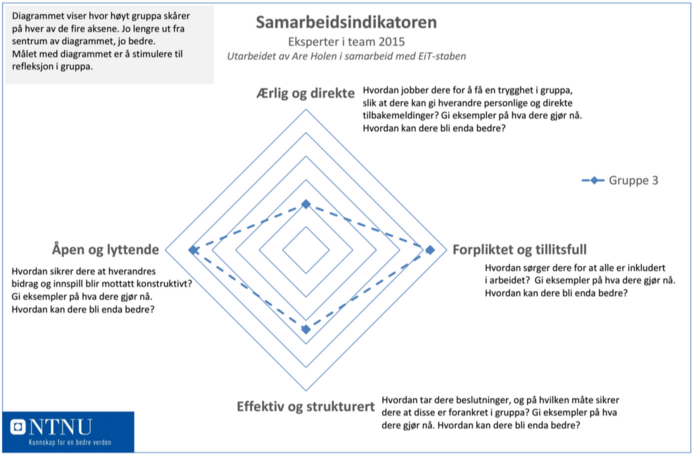
\includegraphics[width=0.5\textwidth]{samarbeidsindikator1.png}
\end{center}

\paragraph{Sosiale inntrykk}

En god sosial kommunikasjon og en god tone i gruppen hjelper til for å skape et positiv og trygt arbeidsmiljø.
Det gir medlemmer mer lyst til å samarbeide, og de føler seg mer komfortable med å jobbe sammen.
Et godt sosialt miljø i gruppen gjorde at medlemmene ble mer klare over hvilke personlighetstyper som fins i gruppen, noe som er svært viktig informasjon i et samarbeid.
Fra begynnelsen av prossessen har hvert enkelt gruppemedlem vært inkluderende og dedikert. 
Derfor ble, for eksempel, innsjekk og utsjekk alltid tatt på alvor.
I disse samlingene har individer fått mulighet til å vise tillit til hverandre og inkludere resten av gruppen i sitt liv. 
Det ble etterhvert en slags tradisjon, hvor vi følger hverandres prosjekt og ikke minst utvikling i andre området av livet.
Crossfit, barn, maraton, røyking, Bahamas, mat og Samfundet er noen temaer som har vært gjennomgått.

At gruppen har hatt så vennlig sosial kontakt medfører til både positive og negative konsekvenser.
Det positive er at samtlige gruppenmedlemmer ble motivert fra begynnelsen til å delta og gjøre en god innsats.
Ikke minst var det viktig for å bevare den gode tonen samt unngå eventuelle konflikter.
En naturlig konsekvens av dette er at medlemmer kanskje ikke tør å ødelegge den positive stemningen ved å gi hverandre for direkte tilbakemeldinger eller kritikk i sammenheng med arbeidet.
Kanskje er det dette fenomenet samarbeidsindikatoren adresserer når den viser at gruppen av vært lite ærlig og direkte.
Den gode tonen gjorde også at gruppen i begynnelsen har slitt noe med tid og struktur og tapte derfor på effektivitet.

Stemningen i gruppen har stort sett vært avslappet med tendenser til vitsing.
Det ble raskt tendenser til distraksjoner under gruppemøter, og behovet for å kalle til ro dukket opp ved flere anledninger, noe som førte til at gruppen innførte ordstyrer.

Det er ingen tvil om at sosialt god kommunikasjon går hånd i hånd med hvordan medlemmer jobber.
Siden alle har vært svært dediktert i arbeidet sitt og etterhvert fått tillit fra gruppen, fikk gruppen sigende et mer avslappende forhold til forsinkelser, fravær og fristforsinkelser.

Medlemmenes inkludering av hverandre og positive forhold til faget gjorde at medlemmene følte eierskap og ansvar i samarbeidet.
Samtlige medlemmer ble sett og hørt, og ingen fikk mulighet til å melde seg ut.
Gruppen har for eksempel bestemt seg for å dra på restaurant for å ferie sammen når rapportene er leverte. 
Det gjør at medlemmene er knyttet sammen og deler ansvar.
Å fokusere på at alt skulle gjøres sammen i sosial sammenheng har hatt positiv konsekvens i det faglige arbeidet.
\iffalse
(Eksempel av Jonas i konferans [forelesningen?] som satt alene, Karsten og Anna gjorde plass sånn at de kunne alle 3 sitte sammen, Crossfit dag, vi slette å ta ut en medlem av gruppe )


<Kort beskrivelse av den sosiale atmosfæren: Avslappet, tendens til vitsing, tendens til distractions under gruppemøter, tendens til å kalle til fokus når det trengs>
etc
Spørsmål:
Har vi hatt positiv innflytelse av at alle var villige til å gjøre en grundig jobb (gå etter A’en, samarbeidskontrakten)?
Var alle det fra start av, eller kom viljen til å gjøre en grundig jobb som følge av god teamfølelse?
“Veldig avslappet” pros and cons
Pros: Har dette gjort at folk ikke blir arrige over forseintkomminger og fristoverskridelser, i og med at alle på teamet føler seg trygge på at en innsatts blir gjort? 
Pros: Har dette gjort det lettere å håndtere uenigheter, siden folk har hatt god vilje og “likt” hverandre?
Har det vært nyttig som ‘sosial judo’ i å kunne snakke om konflikter i tidlig fase, lenge før kokepunkt?
Cons: Har det kostet oss verdiful tid, spesielt i den første halvdelen av faget? Var progresjon i arbeidet jevnlig handicappet? Gikk det ofte veldig sakte fremover? Brukte gruppen mye tid på unødvendig sosial prat? Kunne dette føre til frustrasjon blandt noen medlemmer på gruppen, og mindre hos andre, derved skape mulighet for konflikt (noen jobber hardt, andre prater bare tull)
Innflytelse av god sosial stemning på innsjekk/utsjekk: bryr folk seg om hverandre (referer til fagets beskrivelse av forskjellige team-egenskaper). F eks teamet bryr seg om de individuelle og hvilken overføringsverdi dette har til arbeidet.
 Anna røykestopp/maraton, Simen + sønn Odin, Ingelin CF progresjon, Martin mat (:))) /DJing/tech ansvar på singsaker studenthjem), Karsten mountainbike/Bahamastur, Jonas sine eventyr på samfundet 

<mangler spesifikke referanser til referat; vi må få samlet disse et sted>

\fi
